\chapter{Parallax}


{\bf Introduction.}

Parallax is the method used to find the distances to the closest
stars.  It is the first step in the ``distance ladder'' used to find
distances to other stars and ultimately to other galaxies.  In this
lab you will use the method of parallax to determine the distance to a
nearby object: one of the classroom windows.

Here's the big idea behind parallax measurements.  Suppose you want
to measure the distance to the star in the drawing on the next page.  
You observe
the apparent position of the star from two locations A and B.  The directions
you have to look in order to see the object from the two locations
are slightly different, and the amount of difference can be represented
by the angle $\theta$.  If you can determine $\theta$, then you can
use the small-angle formula to determine the distance to the object.

The small-angle formula says that
$$
s = \left(2\pi\over 360^\circ\right)\theta D.
$$
Here $s$ is the distance between the two observation points, and 
$D$ is the distance to the object.\footnote{This is the version 
of the small-angle formula that has $\theta$ in degrees.  That's
the version that's most useful in this lab.  If you measure angles
in arc-seconds instead, then you use the version of the
formula that has the number $206\,265$ in it.}

(By the way, when we first learned the small-angle formula, we said
that $s$ was the separation between two different objects being
observed, not the separation between two different observation points.
We're now applying the formula to a different situation, but since the
geometrical setup is the same, the same formula works.)

The next question is how to measure $\theta$.  {\it In principle}, we could
measure $\theta$ like this:
\begin{enumerate}
\item Put the telescope at point A and point it at the star.
\item Move the telescope from point A to point B, being {\it very careful}
not to rotate it as you move it.
\item Once the telescope is at point B, rotate it until it is again pointing
at the star.  Measure the angle through which you had to turn the
telescope.  This is $\theta$.
\end{enumerate}
Here's a picture of the various angles:

\centerline{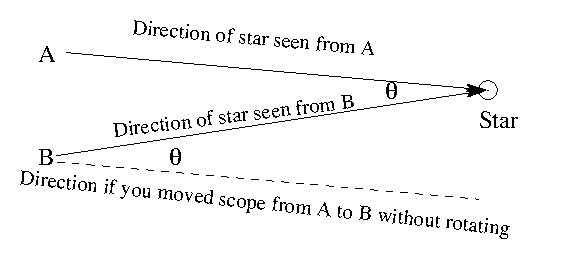
\includegraphics[width=4in]{figs/parallax.eps}}

Although there is nothing wrong with this method in principle,
in practice it's quite inaccurate.  The reason is step 2: it's very hard
to make sure that you didn't jostle the telescope and rotate it just a little
bit when you were moving it.  Since parallax angles are very small, even
a slight error in this step will ruin the method.  So {\it the method above
is no good in practice}.

To make the method work, we need to measure the shift in the angular
position of the star by comparing it to some much more distant background
objects.  Here's the idea:
\begin{enumerate}
\item Put the telescope at point A.  Point the telescope at the
star.
\item Rotate the telescope until it points at a particular {\it background
object}.  Measure the angle through which you had to turn the telescope
to do this.  The result is the {\it angular separation} between the
star and the background object.  Let's call this angle $\alpha$.
\item Move the telescope to point B (without worrying about whether
you're rotating it as you go).
\item Point the telescope at the star, then at the same background
object as before.  Measure the angular separation this time, and call
it $\beta$.
\item The parallax angle $\theta$ is just the difference between
$\alpha$ and $\beta$.
\end{enumerate}
The picture below illustrates the various angles in this
method.  The main point is that
the background object is presumed to be extremely far away (much further
than the star).  This means that the lines of sight to the background
object from the two locations are essentially parallel to each other.

\centerline{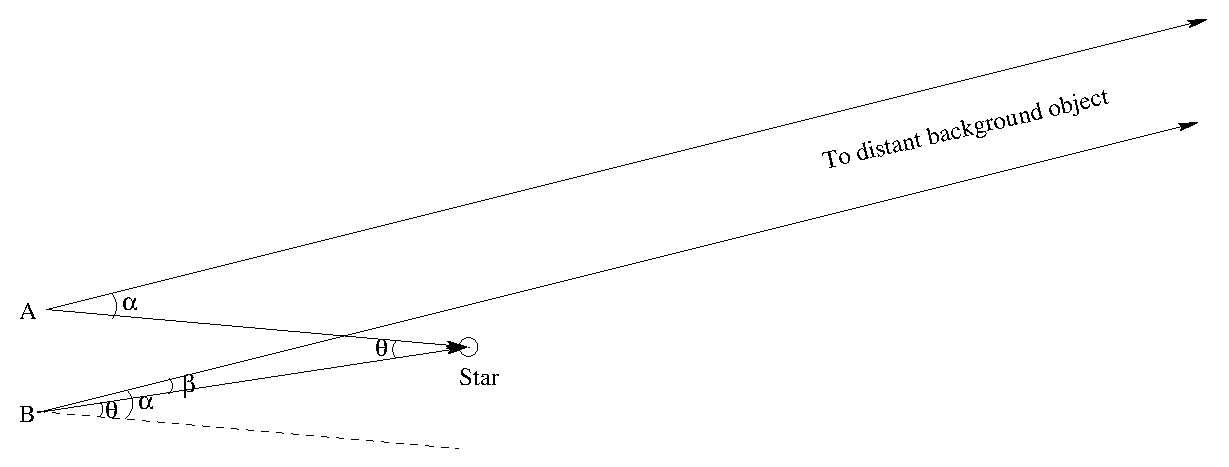
\includegraphics[width=6in]{figs/parallax2.eps}}


\bigskip

{\bf Procedure.}

The ``star'' in this lab will be the vertical divider separating
two panes of the windows at the side of the classroom.  Arrange
the telescopes so that you have a clear view of the ``star.''
Put down a couple of pieces of masking tape to mark the location
of the telescope.  You'll need these later when you determine
how far you moved the telescope.  You can mark the locations
of any convenient points on the telescope base.

(Incidentally, the telescopes we're using here are the ones on the
spectroscopes.  We're not using the ``slit'' side of the spectroscopes
at all in this lab; we're just using the ``telescope'' side.  So 
just set up the apparatus so that the slit is off out of the way, and
ignore it.)

Rotate the telescope until the ``star'' is centered in the field of view.
Use the crosshairs to make sure it's lined up accurately.
Record the angle made by the telescope.  If you forget how to read
the Vernier scale on the telescope base, ask me.

\vskip 1in

Look through the telescope, and choose a faraway ``reference object.''
This should be something easily identifiable and far away (outside
of the building, and preferably across the street).  It should also
be close to, but not quite, the same direction as the ``star.''
Good choices are tree trunks, signs, or lamp posts.

Rotate the telescope until the reference object is centered on the crosshairs,
and record the angle made by the telescope now.

\vskip 1in

Subtract these two angles from each other.  The result is $\alpha$,
the angular separation between the ``star'' and the reference
object.  (If I were you, I would convert the angles from degrees
and minutes into a decimal number of degrees before subtracting.
For instance, I'd convert $42^\circ\ 20'$, into $42.33^\circ$,
by using the fact that a minute is $1\over 60$ of a degree.)

\vskip 1in

Move the telescope over about 15 centimeters or so.  (The exact amount
doesn't matter.)  Move it in a direction perpendicular to the direction
of the ``star,'' not towards or away from the star.
Mark the new position with masking tape again.

Look through the telescope.  You should notice that the position
of the ``star'' relative to the background objects has shifted
a bit.  That's parallax.

Repeat the procedure above: Measure the angular position of the
star and the angular position of the reference object (same object
as last time!).  

\vskip 2.5in

What is the parallax angle $\theta$?

\vskip 1in

Using a ruler and your masking-tape marks, measure the distance between
the two observation points A and B.

\vskip 1in

Now you have all the information you need to determine the distance to
the ``star.''  What is it?

\vskip 1in

Use a tape measure to determine the actual distance.

\vskip 1in

Do you think your results are reasonably accurate?  What
do you think the main sources of error are in this method?






